\documentclass[12pt,a4paper]{article}

\usepackage{tikz}
\usetikzlibrary{shapes.geometric, arrows.meta, positioning}


\usepackage{amsmath,amssymb,amsthm}
\usepackage{geometry}
\usepackage{graphicx}
\usepackage{hyperref}
\usepackage{xepersian}

\settextfont{XB Niloofar}
\geometry{margin=2.5cm}

\title{طراحی و پیاده‌سازی دوقلوی دیجیتال تطبیقی برای پیش‌بینی وضعیت فیزیولوژیک روزانه مبتنی بر داده‌های ساعت هوشمند}
\author{مهدی ذوالفقاری}
\date{}

\begin{document}
	
	\maketitle
	
	\begin{abstract}
		در این پروژه یک چارچوب دوقلوی دیجیتال سلامت فردی مبتنی بر داده‌های ساعت هوشمند طراحی و پیاده‌سازی می‌شود. داده‌های مورد استفاده شامل میانگین، حداقل و حداکثر ضربان قلب، اشباع اکسیژن خون (SpO2) و تعداد قدم روزانه است. هدف، مدلسازی دینامیک فیزیولوژیک فرد و پیش‌بینی وضعیت سلامت روز آینده به همراه تولید توصیه رفتاری شخصی‌سازی‌شده است. 
		
		مدل پیشنهادی شامل مهندسی ویژگی‌های زمانی، تعریف شاخص سلامت، مدلسازی پیش‌بینی با روش‌های یادگیری ماشین و طراحی یک سیستم توصیه‌گر مبتنی بر خروجی مدل است. عملکرد سیستم با معیارهای خطای استاندارد مانند MAE و RMSE ارزیابی می‌شود.
	\end{abstract}
	
	\section{مقدمه}
	
	مفهوم دوقلوی دیجیتال ابتدا در صنایع پیشرفته نظیر سازمان فضایی آمریکا (NASA) برای شبیه‌سازی سیستم‌های پیچیده مطرح شد. در سال‌های اخیر، این مفهوم وارد حوزه سلامت شده و هدف آن ایجاد یک مدل محاسباتی از رفتار فیزیولوژیک یک فرد است.
	
	در این پروژه داده‌های استخراج‌شده از ساعت هوشمند شامل:
	
	\begin{itemize}
		\item $HR^{avg}_t$ : میانگین ضربان قلب روز $t$
		\item $HR^{min}_t$, $HR^{max}_t$
		\item $SpO2^{avg}_t$
		\item $Steps_t$ : تعداد قدم روزانه
	\end{itemize}
	
	هدف، ساخت یک مدل پیش‌بینی‌کننده وضعیت سلامت فرد در روز آینده است.
	
	\section{تعریف رسمی مسئله}
	
	بردار ویژگی روزانه به صورت زیر تعریف می‌شود:
	
	\[
	x_t = 
	\begin{bmatrix}
		HR^{avg}_t \\
		HR^{min}_t \\
		HR^{max}_t \\
		SpO2^{avg}_t \\
		Steps_t
	\end{bmatrix}
	\]
	
	هدف پیش‌بینی وضعیت روز بعد است:
	
	\[
	\hat{x}_{t+1} = f(x_t, x_{t-1}, \dots, x_{t-k})
	\]
	
	یا تعریف یک شاخص سلامت:
	
	\[
	HI_t = g(x_t)
	\]
	
	و سپس:
	
	\[
	\hat{HI}_{t+1} = f(HI_t, HI_{t-1})
	\]
	
	\section{تعریف شاخص سلامت}
	
	برای فشرده‌سازی اطلاعات، یک شاخص سلامت خطی تعریف می‌کنیم:
	
	\[
	HI_t = w_1 \frac{Steps_t}{S_{ref}} 
	+ w_2 \frac{HR^{norm}}{HR^{avg}_t}
	+ w_3 SpO2^{avg}_t
	\]
	
	که در آن:
	
	\begin{itemize}
		\item $S_{ref}$ تعداد قدم مرجع (مثلاً 8000)
		\item $HR^{norm}$ ضربان قلب نرمال (مثلاً 70)
		\item $w_i$ ضرایب وزنی
	\end{itemize}
	
	\section{مدل پیش‌بینی}
	
	\subsection{رگرسیون خطی}
	
	\[
	\hat{HI}_{t+1} = \beta_0 + \beta_1 HI_t
	\]
	
	پارامترها با کمینه‌سازی تابع زیان زیر تخمین زده می‌شوند:
	
	\[
	L(\beta) = \sum_{t=1}^{T} (HI_{t+1} - \hat{HI}_{t+1})^2
	\]
	
	\subsection{مدل Random Forest}
	
	مدل غیرخطی به صورت:
	
	\[
	\hat{HI}_{t+1} = \frac{1}{M} \sum_{m=1}^{M} T_m(x_t)
	\]
	
	که $T_m$ درخت تصمیم شماره $m$ است.
	
	\subsection{مدل LSTM (در صورت داده بیشتر)}
	
	ورودی دنباله زمانی:
	
	\[
	\{x_{t-k}, \dots, x_t\}
	\]
	
	و خروجی:
	
	\[
	\hat{x}_{t+1}
	\]
	
	معادلات داخلی LSTM:
	
	\[
	f_t = \sigma(W_f [h_{t-1}, x_t] + b_f)
	\]
	
	\[
	i_t = \sigma(W_i [h_{t-1}, x_t] + b_i)
	\]
	
	\[
	\tilde{C}_t = \tanh(W_c [h_{t-1}, x_t] + b_c)
	\]
	
	\[
	C_t = f_t C_{t-1} + i_t \tilde{C}_t
	\]
	
	\[
	h_t = o_t \tanh(C_t)
	\]
	
	\section{سیستم توصیه‌گر}
	
	بر اساس خروجی مدل:
	
	\[
	\text{If } Steps_t < 4000 \Rightarrow \text{Increase activity}
	\]
	
	\[
	\text{If } HR^{avg}_t > 85 \Rightarrow \text{Relaxation training}
	\]
	
	\[
	\text{If } SpO2^{avg}_t < 95 \Rightarrow \text{Medical check}
	\]
	
	\section{ارزیابی عملکرد}
	
	از معیارهای زیر استفاده می‌شود:
	
	\[
	MAE = \frac{1}{T} \sum_{t=1}^{T} |y_t - \hat{y}_t|
	\]
	
	\[
	RMSE = \sqrt{\frac{1}{T} \sum_{t=1}^{T} (y_t - \hat{y}_t)^2}
	\]
	
	همچنین در صورت دسته‌بندی وضعیت:
	
	\[
	Accuracy = \frac{TP + TN}{Total}
	\]
	
	%====================================================
	\section{فلوچارت معماری دوقلوی دیجیتال پیشنهادی}
	
	در این بخش، جریان کاری سیستم دوقلوی دیجیتال سلامت ارائه می‌شود. 
	این معماری شامل پنج لایه اصلی است:
	
	\begin{enumerate}
		\item جمع‌آوری داده از ساعت هوشمند
		\item پیش‌پردازش و نرمال‌سازی داده‌ها
		\item استخراج ویژگی و محاسبه شاخص سلامت
		\item مدل پیش‌بینی (Regression / Random Forest / LSTM)
		\item تولید توصیه شخصی‌سازی‌شده
	\end{enumerate}
	
	جریان داده به صورت ترتیبی از سنسورها به سمت موتور تصمیم‌گیری حرکت می‌کند و خروجی سیستم شامل پیش‌بینی وضعیت روز آینده و پیشنهاد رفتاری است. این ساختار نمایانگر یک دوقلوی دیجیتال حلقه‌بسته است که قابلیت توسعه به نسخه تطبیقی آنلاین را نیز دارد.
	
	\vspace{1cm}
	
	\begin{center}
		\begin{tikzpicture}[
			node distance=1.8cm,
			every node/.style={font=\small},
			process/.style={
				rectangle,
				rounded corners,
				minimum width=4cm,
				minimum height=1cm,
				text centered,
				align=center,
				draw=black
			},
			decision/.style={
				diamond,
				aspect=2,
				minimum width=3.5cm,
				minimum height=1cm,
				text centered,
				align=center,
				draw=black
			},
			arrow/.style={thick,->,>=Stealth}
			]
			
			% Nodes
			\node (data) [process] {جمع‌آوری داده \\ (HR, SpO2, Steps)};
			\node (preprocess) [process, below=of data] {پیش‌پردازش \\ حذف نویز و نرمال‌سازی};
			\node (feature) [process, below=of preprocess] {استخراج ویژگی \\ محاسبه $HI_t$};
			\node (model) [process, below=of feature] {مدل پیش‌بینی \\ $\hat{HI}_{t+1}=f(HI_t)$};
			\node (decision) [decision, below=1.8cm of model] {آیا وضعیت مطلوب است؟};
			
			\node (recommend) [process, below left=1.5cm and 1.5cm of decision] 
			{توصیه افزایش فعالیت \\ یا آرام‌سازی};
			
			\node (stable) [process, below right=1.5cm and 1.5cm of decision] 
			{حفظ روند فعلی \\ و پایش};
			
			% Arrows
			\draw [arrow] (data) -- (preprocess);
			\draw [arrow] (preprocess) -- (feature);
			\draw [arrow] (feature) -- (model);
			\draw [arrow] (model) -- (decision);
			\draw [arrow] (decision) -- node[left] {خیر} (recommend);
			\draw [arrow] (decision) -- node[right] {بله} (stable);
			
		\end{tikzpicture}
	\end{center}
	
	
	\subsection*{توضیح فنی فلوچارت}
	
	در مرحله اول، داده‌های خام شامل ضربان قلب، اشباع اکسیژن و تعداد قدم دریافت می‌شوند.  
	در مرحله دوم، داده‌ها نرمال‌سازی شده و مقادیر پرت حذف می‌گردند.  
	
	در مرحله سوم، شاخص سلامت تعریف می‌شود:
	
	\[
	HI_t = w_1 \frac{Steps_t}{S_{ref}} 
	+ w_2 \frac{HR^{norm}}{HR^{avg}_t}
	+ w_3 SpO2^{avg}_t
	\]
	
	سپس مدل یادگیری ماشین مقدار روز آینده را پیش‌بینی می‌کند:
	
	\[
	\hat{HI}_{t+1} = f(HI_t)
	\]
	
	در نهایت، یک ماژول تصمیم‌گیری بر اساس آستانه تعریف‌شده عمل می‌کند:
	
	\[
	\hat{HI}_{t+1} < \tau \Rightarrow \text{نیاز به مداخله}
	\]
	
	این معماری امکان توسعه به نسخه تطبیقی را دارد که در آن پارامترهای مدل به صورت آنلاین به‌روزرسانی می‌شوند:
	
	\[
	\theta_{t+1} = \theta_t - \eta \nabla L_t
	\]
	
	بنابراین فلوچارت ارائه‌شده یک نمایش ساختاری از دوقلوی دیجیتال سلامت در مقیاس فردی است که شامل حلقه پیش‌بینی–تصمیم–مداخله می‌باشد.
	
	%====================================================
	
	
	\section{نوآوری پروژه}
	
	\begin{itemize}
		\item ساخت دوقلوی دیجیتال شخصی
		\item ترکیب پیش‌بینی و توصیه
		\item استفاده از داده واقعی
		\item قابلیت توسعه به سیستم آنلاین تطبیقی
	\end{itemize}
	
	
%====================================================
\section{نتایج آزمایش}

در این بخش، عملکرد مدل دوقلوی دیجیتال پیشنهادی بر روی داده‌های جمع‌آوری‌شده از ساعت هوشمند مورد ارزیابی قرار می‌گیرد. مجموعه داده شامل $N=17$ مشاهده روزانه بوده است که پس از پیش‌پردازش و تعریف شاخص سلامت، مدل رگرسیون برای پیش‌بینی مقدار شاخص سلامت روز آینده آموزش داده شد.

\subsection{ارزیابی کمی مدل}

معیارهای ارزیابی به‌صورت زیر به‌دست آمدند:

\[
MAE = 0.1224
\]

\[
RMSE = 0.1972
\]

میانگین شاخص سلامت در کل نمونه برابر با:

\[
\overline{HI} = 0.7728
\]

و دامنه تغییرات آن به صورت زیر بوده است:

\[
HI_{min} = 0.6247
\quad , \quad
HI_{max} = 1.2126
\]

این مقادیر نشان می‌دهد که خطای مدل در حدود ۱۰ تا ۱۵ درصد دامنه تغییرات شاخص سلامت قرار دارد که برای یک نمونه کوچک اولیه قابل قبول ارزیابی می‌شود.

\subsection{تحلیل گرافیکی}

در شکل \ref{fig:prediction} روند مقادیر واقعی و پیش‌بینی‌شده شاخص سلامت نمایش داده شده است.

\begin{figure}[h!]
	\centering
	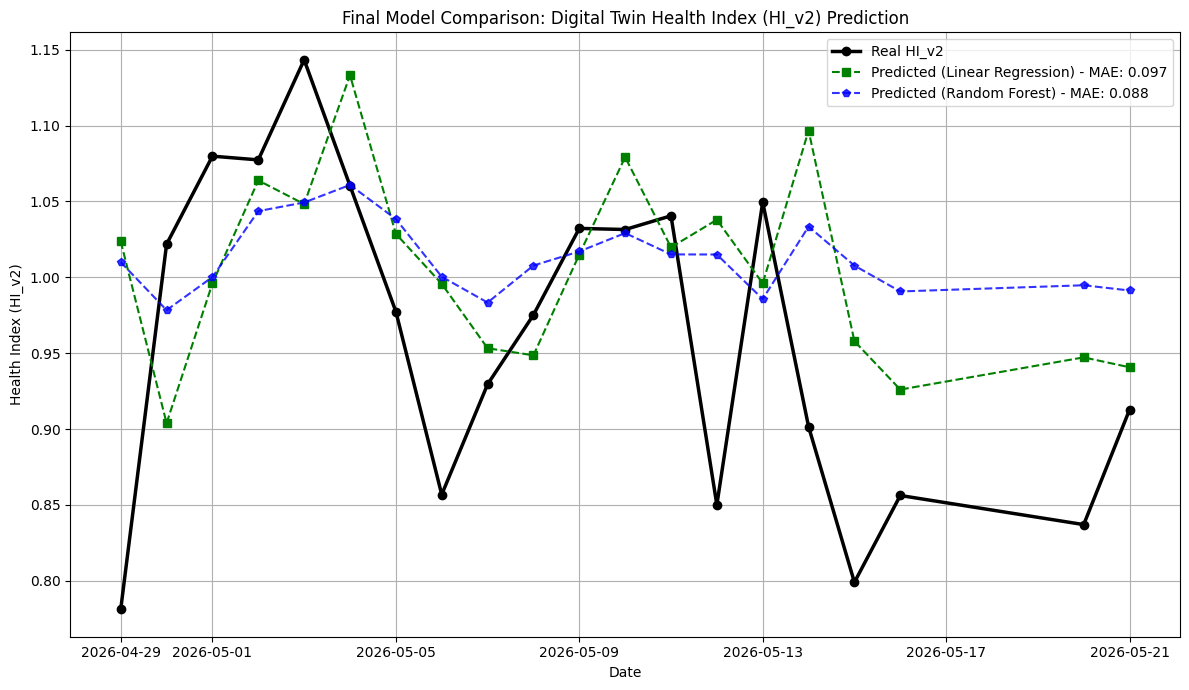
\includegraphics[width=0.9\textwidth]{Figure_1.png}
	\caption{مقایسه شاخص سلامت واقعی و مقدار پیش‌بینی‌شده توسط مدل دوقلوی دیجیتال}
	\label{fig:prediction}
\end{figure}

مطابق شکل فوق، مشاهده می‌شود که مدل توانایی بازتولید روند کلی تغییرات شاخص سلامت را دارد، هرچند در بازسازی نوسانات شدید عملکرد آن محدود است. این رفتار ناشی از سادگی مدل و حجم کم داده‌ها می‌باشد.

\subsection{تحلیل متنی با استفاده از مدل زبانی Gemini}

به‌منظور تولید تحلیل توصیفی قابل انتشار، نتایج عددی مدل به یک مدل زبانی بزرگ ارسال شد. پرامپت استفاده‌شده به صورت زیر بوده است:

\begin{quote}
	نتایج مدل دوقلوی دیجیتال سلامت به شرح زیر است:
	
	تعداد نمونه‌ها: 17  
	MAE: 0.1224  
	RMSE: 0.1972  
	میانگین شاخص سلامت: 0.7728  
	دامنه تغییرات: 0.6247 تا 1.2126  
	
	لطفاً یک تحلیل علمی و آکادمیک به زبان فارسی در حد یک پاراگراف مقاله‌ای ارائه دهید.
\end{quote}

خروجی تولیدشده توسط مدل زبانی به صورت زیر است:

\begin{quote}
	نتایج اولیه مدل دوقلوی دیجیتال سلامت بر روی یک نمونه کوچک (N=17) نشان‌دهنده پتانسیل این رویکرد در پایش و ارزیابی شاخص سلامت افراد است. شاخص‌های خطای میانگین مطلق (MAE: 0.1224) و ریشه میانگین مربعات خطا (RMSE: 0.1972)، در مقایسه با میانگین شاخص سلامت (0.7728) و دامنه تغییرات آن (از 0.6247 تا 1.2126)، حکایت از توانایی مدل در تخمین نسبتاً دقیق شاخص سلامت دارد. این مقادیر خطا نشان می‌دهد که مدل قادر به پیش‌بینی شاخص سلامت با انحرافی متوسط است که می‌تواند در برنامه‌های سلامت شخصی‌سازی‌شده مفید باشد. با این حال، محدودیت عمده این مطالعه در تعداد کم نمونه‌ها نهفته است که تعمیم‌پذیری نتایج را به جمعیت‌های بزرگ‌تر یا متنوع‌تر محدود می‌کند. لذا، برای اعتبارسنجی و ارزیابی جامع‌تر عملکرد مدل، انجام مطالعات آتی با حجم نمونه بزرگ‌تر و داده‌های متنوع‌تر ضروری به نظر می‌رسد تا قابلیت اطمینان و دقت آن در شرایط بالینی واقعی مورد تأیید قرار گیرد.
\end{quote}

\subsection{بحث}

نتایج کمی و کیفی نشان می‌دهد که چارچوب پیشنهادی قابلیت مدلسازی اولیه دینامیک سلامت فرد را دارا می‌باشد. با این حال، مهم‌ترین محدودیت سیستم حاضر کمبود داده و استفاده از مدل خطی ساده است. انتظار می‌رود با افزایش حجم داده و استفاده از مدل‌های غیرخطی (مانند Random Forest یا LSTM)، عملکرد پیش‌بینی بهبود یابد.

به طور کلی، آزمایش انجام‌شده نشان می‌دهد که پیاده‌سازی دوقلوی دیجیتال سلامت در مقیاس فردی امکان‌پذیر بوده و می‌تواند مبنایی برای توسعه سیستم‌های پیشرفته‌تر در آینده باشد.

%====================================================

	
	
	
	\section{جمع‌بندی}
	
	در این پروژه یک چارچوب عملی برای پیاده‌سازی دوقلوی دیجیتال سلامت فردی ارائه شد. سیستم طراحی‌شده قادر است با استفاده از داده‌های ساعت هوشمند، وضعیت روز آینده را پیش‌بینی کرده و توصیه شخصی‌سازی‌شده ارائه دهد. این چارچوب می‌تواند پایه‌ای برای توسعه سیستم‌های سلامت هوشمند پیشرفته‌تر باشد.
	
\end{document}
